% -------------------------------------------------------------------------------- %

\begin{exercise}

The nonplanning method looks particularly poor in Figure \ref{fig:8.3} because it is a one-step method;
a method using multi-step bootstrapping would do better.
Do you think one of the multi-step bootstrapping methods from Chapter 7 could do as well as the Dyna method?
Explain why or why not.

\setcounter{section}{8}
\setcounter{figure}{2}

\begin{figure}[H]
    \centering
    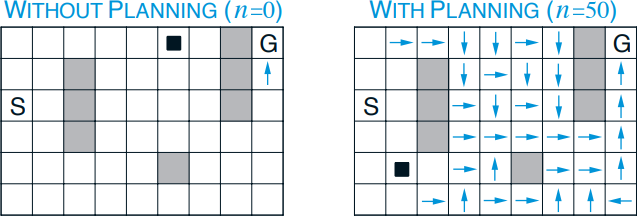
\includegraphics[width = 0.5 \textwidth]{4.45.png}
    \caption
    {
        Policies found by planning and nonplanning Dyna-Q agents halfway through the second episode.
        The arrows indicate the greedy action in each state;
        if no arrow is shown for a state, then all of its action values were equal.
        The black square indicates the location of the agent.
    }
    \label{fig:8.3}
\end{figure}

\end{exercise}

% -------------------------------------------------------------------------------- %

\begin{solution}

As we can see in exercise 44, the multi-step bootstrapping methods do worse then their Dyna counterparts. The $n$-step bootstrapping methods, as their name suggests, base their update on the correct reward of the next $n$ steps and bootstrap the value of the encountered state-action pair $S_{t+1},A_{t+1}$. The Dyna method only does one step updates, they bootstrap only from the next state-action pair, but after the agent has taken one step, they update the values of n previously encountered state-action pairs.

So the $n$-step bootstrapping method looks $n$-steps ahead and bootstraps from that value, the number of updates along the way is the same as the number of episodes. In the Dyna algorithm we only look one step ahead but in every step of the episode we update $n$ of the previously encountered state-action values. So in the Dyna algorithm one update is less accurate, but we update more often, which seems to lead to finding the best transitions faster.
\end{solution}

% -------------------------------------------------------------------------------- %
